\documentclass{beamer}

%%%%%%%%%%%%%%%%%%%%%%%%%%%%%%%%%%%%%%%%%%%%%%%%%%%%%%%%%%%%%%%%
%%%                  Themes and such                         %%%
%%%%%%%%%%%%%%%%%%%%%%%%%%%%%%%%%%%%%%%%%%%%%%%%%%%%%%%%%%%%%%%%
\mode<presentation>
{
%  \usetheme{Copenhagen}  
  \usetheme{Warsaw}  
%  \usetheme{Malmoe}  

  %make my huge toc fit on one slide (and not look horrible)
  \setbeamerfont{subsection in toc}{series=\bfseries}
  \setbeamerfont{subsection in toc}{size=\tiny,series=\bfseries}
}
%\setbeamersize{text margin left=0.5cm,text margin right=0.5cm}

%%%%%%%%%%%%%%%%%%%%%%%%%%%%%%%%%%%%%%%%%%%%%%%%%%%%%%%%%%%%%%%%
%%%                       Packages                           %%%
%%%%%%%%%%%%%%%%%%%%%%%%%%%%%%%%%%%%%%%%%%%%%%%%%%%%%%%%%%%%%%%%
\usepackage{multimedia}
\usepackage{multirow}
\usepackage{xcolor}

% Define commands 

 \newcommand{\half}{\ensuremath{\frac{1}{2}}}

 \newcommand{\bea}{\begin{eqnarray}}
 \newcommand{\eea}{\end{eqnarray}}
 \newcommand{\beq}{\begin{equation}}
 \newcommand{\eeq}{\end{equation}}
 \newcommand{\bed}{\begin{displaymath}}
 \newcommand{\eed}{\end{displaymath}}
\newcommand{\pd}[2]{\frac{\partial #1}{\partial #2}}
\newcommand{\pf}[2]{\frac{d #1}{d #2}}
\newcommand{\pdt}[2]{\frac{\partial^2 #1}{\partial #2^2}}
\newcommand{\pft}[2]{\frac{d^2 #1}{d #2^2}}
\newcommand{\pdtno}[2]{\frac{\partial^2 #1}{\partial #2}}
\newcommand{\pdd}[3]{\frac{\partial^2 #1}{\partial #2 \partial #3}}
\newcommand{\pff}[3]{\frac{d^2 #1}{d #2 d #3}}

%%%%%%%%%%%%%%%%%%%%%%%%%%%%%%%%%%%%%%%%%%%%%%%%%%%%%%%%%%%%%%%%
%%%                     Title Info                           %%%
%%%%%%%%%%%%%%%%%%%%%%%%%%%%%%%%%%%%%%%%%%%%%%%%%%%%%%%%%%%%%%%%

\title[\hspace{-0.2cm} Isogeometric Analysis Using NURBS]
{
  Isogeometric Analysis Using Non-Uniform Rational Bsplines
}

\author[ME6104 Project, K. Boopathy, S. Niranjan Babu, April 2019]
{
  \large {Komahan Boopathy}\\
  \large Siddarth Niranjan Babu \\
}

\institute
{
  \Large {\textbf{ME6104 Computer Aided Design -- Final Project}} \\
  \vspace{0.2in}
  \large Georgia Institute of Technology\\
  School of Aerospace Engineering
}

\date
{
\small \today
}




%%%%%%%%%%%%%%%%%%%%%%%%%%%%%%%%%%%%%%%%%%%%%%%%%%%%%%%%%%%%%%%%
%%%                   Begin Document                         %%%
%%%%%%%%%%%%%%%%%%%%%%%%%%%%%%%%%%%%%%%%%%%%%%%%%%%%%%%%%%%%%%%%

\begin{document}

%%%%%%%%%%%%%%%%%%%%%%%%%%%%%%%%%%%%%%%%%%%%%%%%%%%%%%%%%%%%%%%%
%%%                     Title Page                           %%%
%%%%%%%%%%%%%%%%%%%%%%%%%%%%%%%%%%%%%%%%%%%%%%%%%%%%%%%%%%%%%%%%

\begin{frame}
  \titlepage
\end{frame}

%%%%%%%%%%%%%%%%%%%%%%%%%%%%%%%%%%%%%%%%%%%%%%%%%%%%%%%%%%%%%%%%
%%%                   Table of Contents                      %%%
%%%%%%%%%%%%%%%%%%%%%%%%%%%%%%%%%%%%%%%%%%%%%%%%%%%%%%%%%%%%%%%%
\begin{frame}
  \frametitle{Outline}
  \tableofcontents
\end{frame}

%%%%%%%%%%%%%%%%%%%%%%%%%%%%%%%%%%%%%%%%%%%%%%%%%%%%%%%%%%%%%%%%
%%%                Introduction and Motivation               %%%
%%%%%%%%%%%%%%%%%%%%%%%%%%%%%%%%%%%%%%%%%%%%%%%%%%%%%%%%%%%%%%%%

\section{Introduction and Motivation}

\begin{frame}[allowframebreaks] \frametitle{Introduction and Motivation}

  \begin{itemize}

  \item Finite Element Analysis is one of the most popular numerical methods to find approximate solution of PDEs.

  \item FEA has wide applications in various fields but there is substantial bottleneck between the CAD and FEA fields.
  
  \item Isogeometric analysis simplifies the transition of exact CAD models into analysis and alleviates the issues originating from geometric discontinuities.
  
  \item IGA significantly reduces the design-to-analysis time in comparison to traditional FEA
  
  \item Its fundamental concept is to utilize NURBS not only for the construction of CAD model, but is also used for its mathematical analysis.

\newpage
\begin{figure}
    \begin{center}
    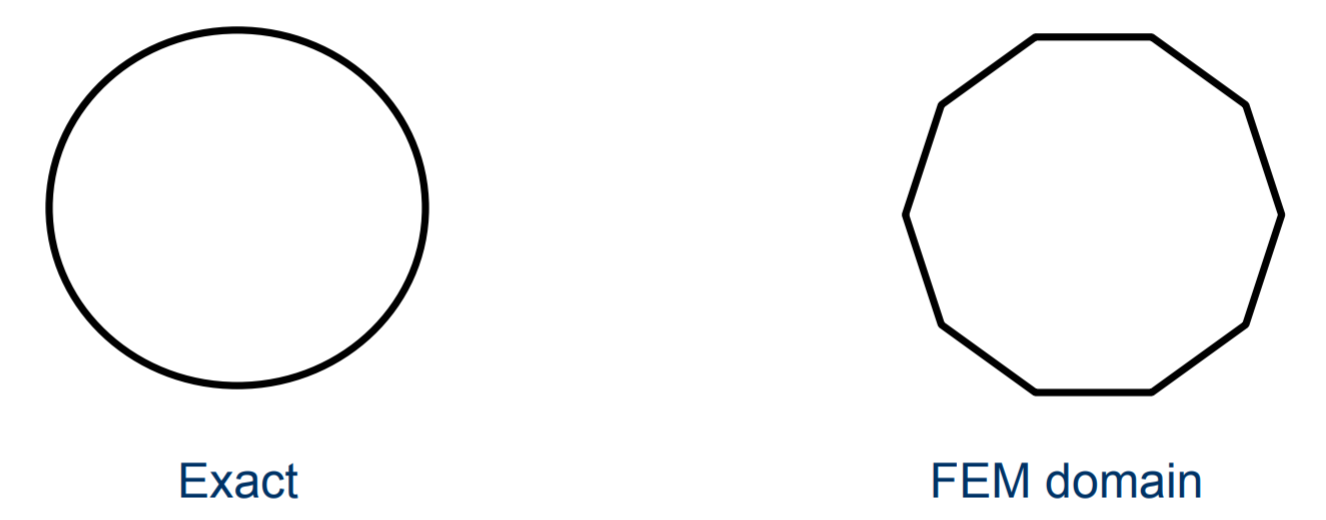
\includegraphics[width=6cm]{figures/exact_vs_fem.PNG}
    \end{center}
    \label{geometry_exact_fem}
\end{figure}
The geometry is described as\\~\\
FEM $\rightarrow$ $x^e=\sum_{i=1}^{n^e}L_ix_i$; \; \; \; \; IGA $\rightarrow$ $x^e=\sum_{i=1}^{n^e_{cp}}R_iP_i$ \\~\\
where, \\
$L_i$ $\rightarrow$ Lagrangian Basis used to represent element in FEM \\
$R_i$ $\rightarrow$ NURBS Basis used to represent element in IGA

\newpage
\begin{center}
\begin{tabular}{cc}
\hline
\hline
 \multicolumn{2}{c}{Differences}\\
\hline
 \footnotesize{FEA} & \footnotesize{IGA} \\
\hline 
 \footnotesize{Nodal Points} & \footnotesize{Control Points} \\
 \footnotesize{Nodal Variables} & \footnotesize{Control Variable}\\
 \footnotesize{Mesh} & \footnotesize{Knots} \\
 \footnotesize{Approximate Geometry} & \footnotesize{Exact Geometry}\\
 \footnotesize{Polynomial Basis} & \footnotesize{NURBS Basis} \\
 \footnotesize{$C^{p-1}$ at inter-element boundary} & \footnotesize{$C^0$ at inter-element boundary } \\
\hline
\hline
\end{tabular}
\end{center}

\item Two static structural problems are chosen to show the potential of Isogeometric Analysis and how it can be the future alternative of FEA.

\end{itemize}
\end{frame}


%%%%%%%%%%%%%%%%%%%%%%%%%%%%%%%%%%%%%%%%%%%%%%%%%%%%%%%%%%%%%%%%%%%%%%
% Analysis of Bar
%%%%%%%%%%%%%%%%%%%%%%%%%%%%%%%%%%%%%%%%%%%%%%%%%%%%%%%%%%%%%%%%%%%%%%

\section{Isogeometric Analysis of 1D-Bar}
\begin{frame}[allowframebreaks] \frametitle{Isogeometric Bar Analysis}

  \begin{columns}
  \begin{column}[b]{0.78\linewidth}
  \begin{block}{Governing Equation}
    \begin{equation}\nonumber
      \pd{}{x} \left( EA \pd{u(x)}{x} \right) - \rho g  = 0
    \end{equation}
    $E$ -- Young's modulus, $A$ -- Area of cross section
  \end{block}
  
  \begin{block}{Solution Form}
    \begin{equation}\nonumber
      u(x) := \sum_{i=1}^{m} N_{i,p}(x) U_i, \quad \pd{u(x)}{x} := \sum_{i=1}^{m} \pd{N_{i,p}(x)}{x}  U_i
    \end{equation}
    $N_{i,p}(x)$ --  NURBS basis functions, $U_i$ -- control points
  \end{block}
  \end{column}
  \begin{column}[b]{0.2\linewidth}
    Deformation of bar  under weight
    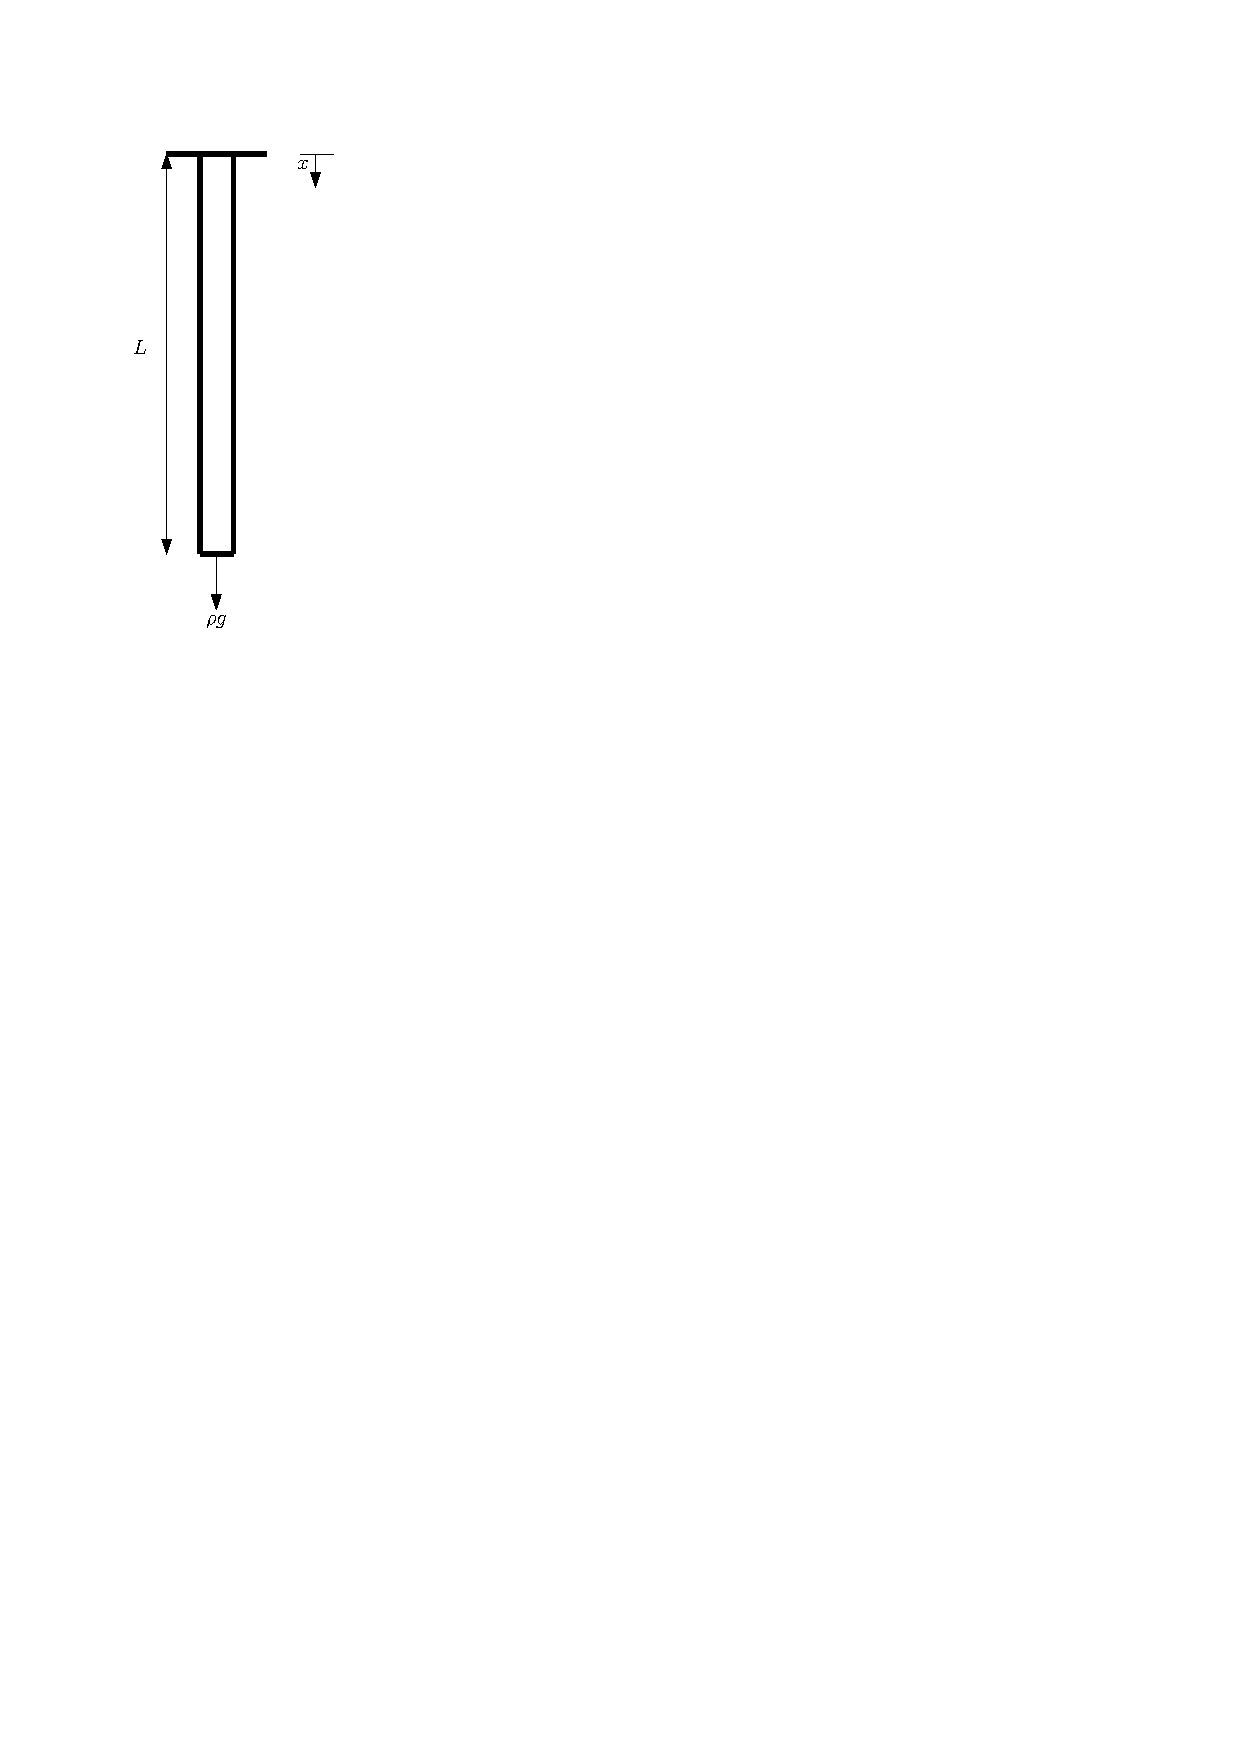
\includegraphics[width=\textwidth]{figures/bar-setup.pdf} 
  \end{column}
  \end{columns}

  \newpage

  \begin{block}{Projection (Galerkin) in Vector Space}
    \begin{equation}\nonumber
      \left\langle  {\color{red}{N_{j,p}(x)}} \bigg\vert {\color{blue}{\pd{}{x} \left[ EA \sum_{i=1}^{m} \pd{N_{i,p}(x)}{x}  U_i  \right]}} \right\rangle  =
      \left\langle  {\color{red}{N_{j,p}(x)}} \bigg\vert {\color{blue}{\rho g}} \right\rangle 
    \end{equation}
  \end{block}
  \begin{block}{Integrating by parts on LHS}
    \begin{equation}\nonumber
      \begin{gathered}
        {{N_{j,p}(x) EA \pd{u(x)}{x}}}  \bigg\vert_{x_a}^{x_b} +  \left\langle {\color{red}{\pd{N_{j,p}(x)}{x}}}  \bigg\vert  {\color{blue}{EA  \pd{N_{i,p}(x)}{x}  U_i}}   \right\rangle \\
        = \\
        \left\langle {\color{red}{N_{j,p}(x)}} \bigg\vert {\color{blue}{\rho g}} \right\rangle \quad \forall j = 1, \ldots,m
      \end{gathered}
    \end{equation}
  \end{block}

  \begin{itemize}
    \item The element matrices and force vector are

\begin{scriptsize}
  \begin{equation}\nonumber
    \setlength\arraycolsep{1.5pt}
    {EA}
    \begin{bmatrix}
      \left \langle {\color{red}{N_1^\prime(x)}} \vert {\color{blue}{N_1^\prime(x)}} \right \rangle &  \left \langle {\color{red}{N_1^\prime(x)}} \vert {\color{blue}{N_2^\prime(x)}} \right \rangle & \left \langle {\color{red}{N_1^\prime(x)}} \vert {\color{blue}{N_m^\prime(x)}} \right \rangle \\
      \left \langle {\color{red}{N_2^\prime(x)}} \vert {\color{blue}{N_1^\prime(x)}} \right \rangle &  \left \langle {\color{red}{N_2^\prime(x)}} \vert {\color{blue}{N_2^\prime(x)}} \right \rangle & \left \langle {\color{red}{N_2^\prime(x)}} \vert {\color{blue}{N_m^\prime(x)}} \right \rangle \\
      \left \langle {\color{red}{N_3^\prime(x)}} \vert {\color{blue}{N_1^\prime(x)}} \right \rangle &  \left \langle {\color{red}{N_3^\prime(x)}} \vert {\color{blue}{N_2^\prime(x)}} \right \rangle & \left \langle {\color{red}{N_3^\prime(x)}} \vert {\color{blue}{N_m^\prime(x)}} \right \rangle \\
    \end{bmatrix}
    \begin{Bmatrix}
      U_1 \\
      U_2 \\
      U_3 \\
    \end{Bmatrix}=
    \begin{Bmatrix}
      \left \langle {\color{red}{N_1(x)}} \vert {\color{blue}{\rho g}} \right \rangle \\
      \left \langle {\color{red}{N_2(x)}} \vert {\color{blue}{\rho g}} \right \rangle \\
      \left \langle {\color{red}{N_3(x)}} \vert {\color{blue}{\rho g}} \right \rangle \\ 
    \end{Bmatrix}    
  \end{equation}
\end{scriptsize}

\item Evaluation of  inner product
  \begin{equation}\nonumber
    \begin{aligned}
      \underset{\text{inner~product}}{\left\langle {\color{red}{f^x(x)}} \big\vert  {\color{blue}{g^x(x)}} \right\rangle} &= \underset{\text{integral}}{\int\limits_{x_a}^{x_b}  {\color{red}{f^x(x)}}  {\color{blue}{g^x(x)}}~dx} &= \underset{\text{quadrature}}{\sum_{k=1}^M \alpha_k^x  {\color{red}{f^x(x_k)}}  {\color{blue}{g^x(x_k)}}}\\
    \end{aligned}
  \end{equation}  

\item Transformation from $x$ to $\xi$ is required as NURBS
  basis is a function of parameter $\xi$
  
  \end{itemize}

  \newpage

  %  \begin{block}{basis}
  \begin{minipage}[b]{0.48\linewidth}
    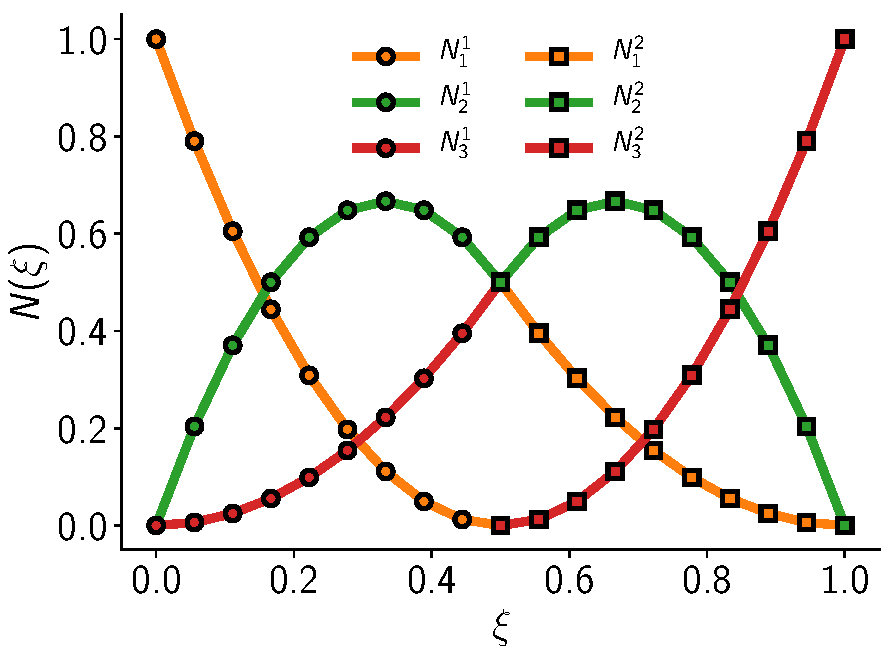
\includegraphics[width=1.0\textwidth]{figures/bar-basis-functions.pdf} \\
    \centering \footnotesize{shapes}
  \end{minipage}
  \begin{minipage}[b]{0.48\linewidth}
    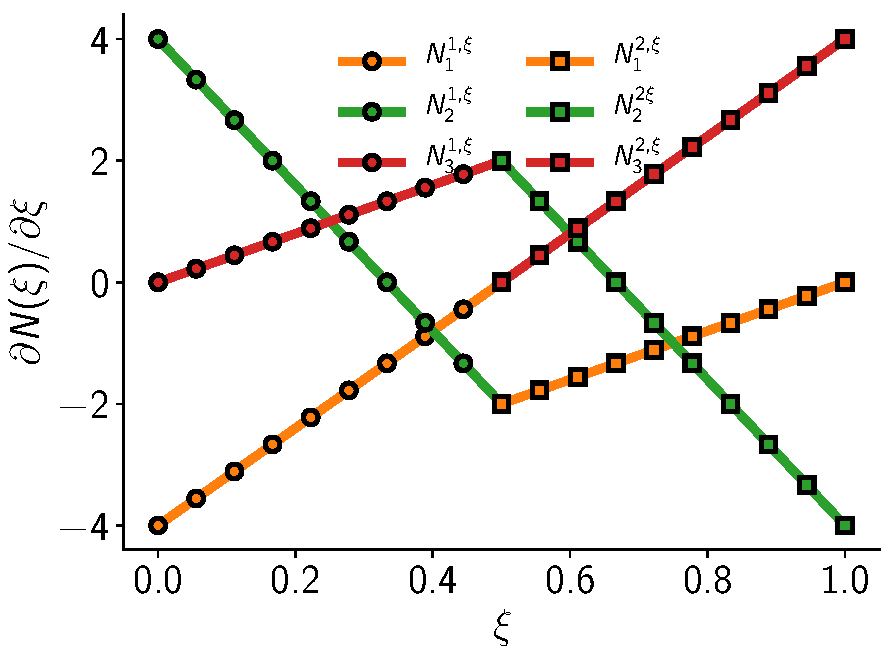
\includegraphics[width=1.0\textwidth]{figures/bar-basis-function-derivatives.pdf} \\
    \centering \footnotesize{derivatives}
  \end{minipage}
  \begin{equation}\nonumber
    \begin{aligned}
       & \textcolor{blue}{\text{element 1 [0,0.5]}}  & & \textcolor{blue}{\text{element 2 [0.5,1]}} \\
      N_1^1(\xi) &=  (2 \xi -1)^2 & N_1^2(\xi) &= (2\xi-2)(\xi-1)  \\
      N_2^1(\xi) &= -2\xi(3\xi-2) &N_2^2(\xi) &= -6\xi^2 + 8\xi -2 \\
      N_3^1(\xi) &=  2\xi^2       & N_3^2(\xi) &= (2\xi -1)^2 \\
    \end{aligned}
  \end{equation}
  % \end{block}
  
  \newpage

  \begin{minipage}{\linewidth}
    \begin{figure}
    \centering
    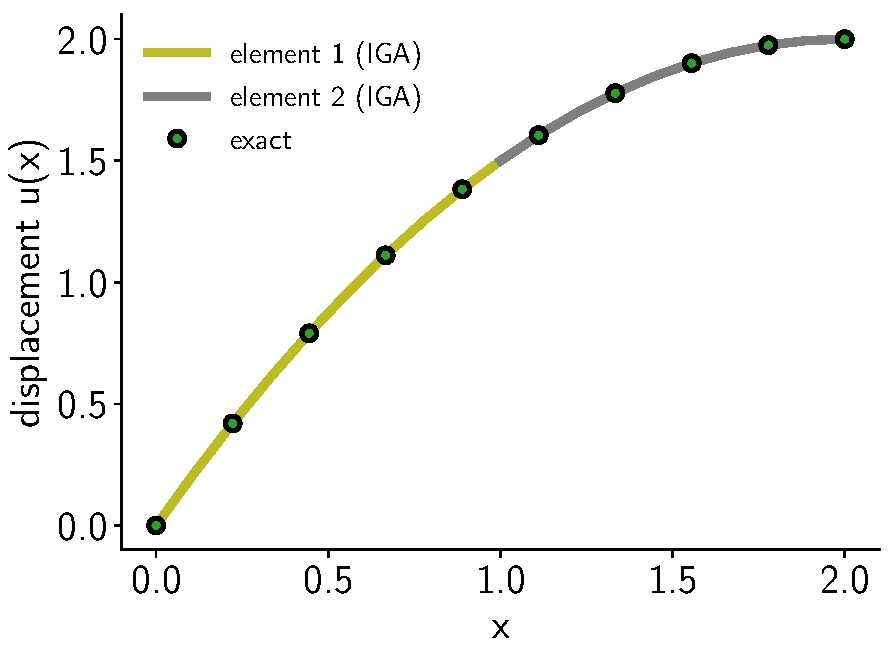
\includegraphics[width=0.5\textwidth]{figures/bar-solution.pdf} \\
    \end{figure}
  \end{minipage}

  \begin{block}{Analytical Solution}
    \begin{equation}\nonumber
      u(x) = \frac{\rho g}{E} \left( Lx - \frac{x^2}{2}\right)
    \end{equation}
  \end{block}

\end{frame}

%%%%%%%%%%%%%%%%%%%%%%%%%%%%%%%%%%%%%%%%%%%%%%%%%%%%%%%%%%%%%%%%%%%%%%
% Analysis of plate
%%%%%%%%%%%%%%%%%%%%%%%%%%%%%%%%%%%%%%%%%%%%%%%%%%%%%%%%%%%%%%%%%%%%%%


\section{Isogeometric Analysis of 2D-Plate}
\begin{minipage}[b]{0.48\linewidth}
    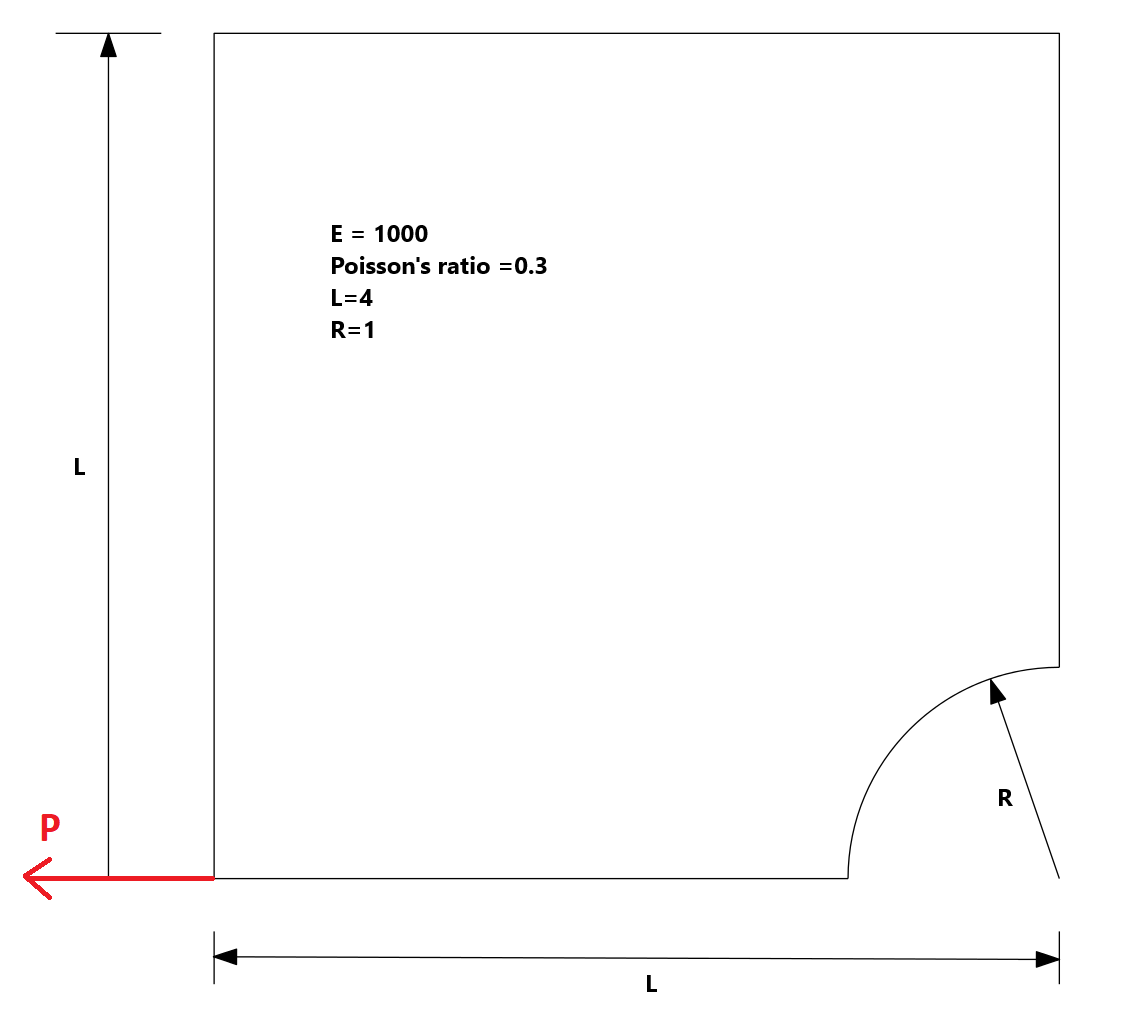
\includegraphics[width=1.0\textwidth,height=0.6\textheight]{figures/plate2.png} \\
    \centering \label{Underformed Plate}
  \end{minipage}
  \begin{minipage}[b]{0.48\linewidth}
    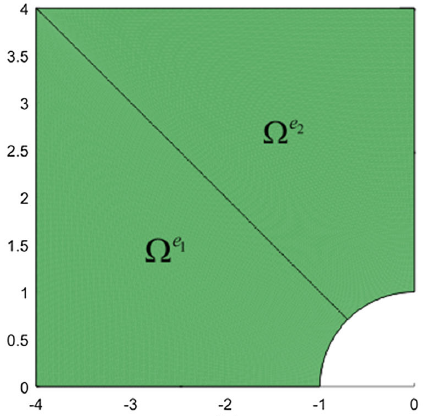
\includegraphics[width=1.0\textwidth,height=0.6\textheight]{figures/plate_elems.PNG} \\
    \centering \label{Deformed Plate}
  \end{minipage}
\begin{itemize}
    \item A plate of L=8 and W=8 with a circular hole is subjected to in-plane concentrated load.

    \item The geometry can be simplified to a quarter plate due to its symmetry. It is modeled using NURBS with 12 control points.
\newpage
  
    \item Divided the geometry into 2 elements and obtained connectivity arrays.
    \item Evaluated the NURBS basis function and its derivatives for all the gauss integration points to obtain strain displacement matrix.
    \begin{equation*}
        B=\begin{bmatrix}
        R_{1,x} & 0 & R_{2,x} & 0 & \dots & R_{9,x} & 0\\
        0 & R_{1,y} & 0 &R_{2,y} & \dots & 0 & R_{9,y}\\
        R_{1,y} & 0 &R_{1,x} &  R_{2,y} & \dots &  R_{9,y} &R_{9,x}
        \end{bmatrix}
    \end{equation*}
    \item B matrix is then used evaluate the element stiffness matrix and force vector with the weak formulation.
    \begin{equation*}
        \int_{\Omega^e} (B^TCB  \,d\Omega)\,u = \int_{\Gamma^e_t} R.t \,d\Gamma +\int_{\Omega^e} R.f \,d\Omega
    \end{equation*}
    \item Assembled the element stiffness and force matrices into the global matrices using connectivity arrays.

      \newpage
  
  \begin{minipage}[b]{0.48\linewidth}
    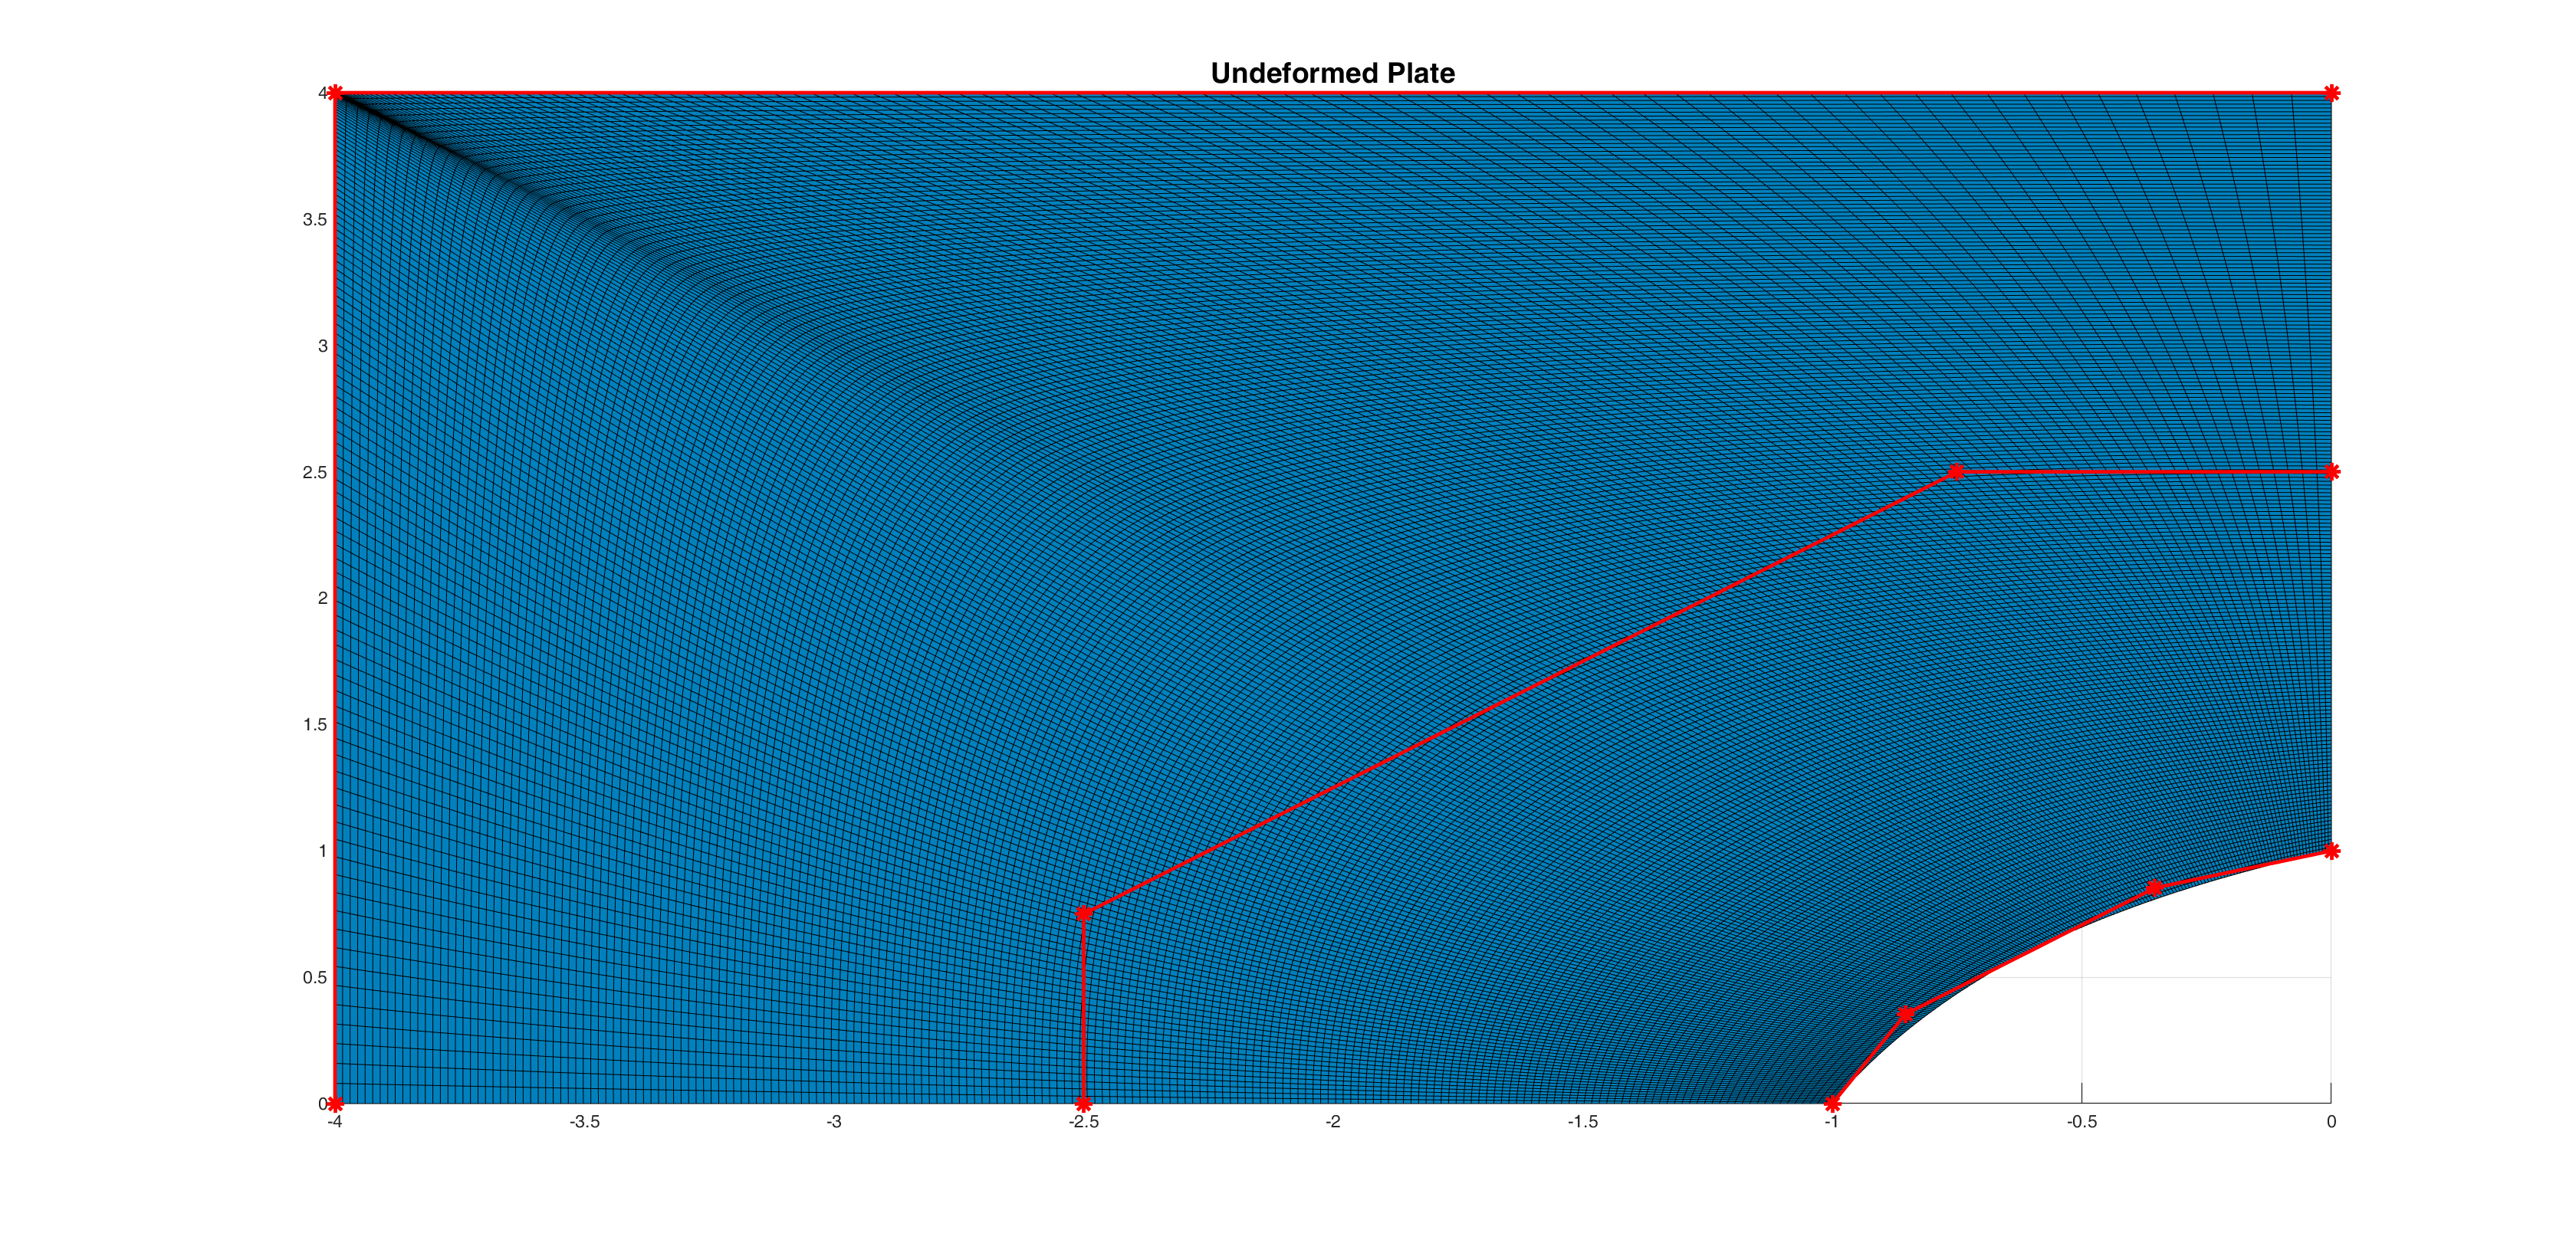
\includegraphics[width=1.0\textwidth,height=0.5\textheight]{figures/undeformed_plate.png} \\
    \centering \label{Underformed Plate}
  \end{minipage}
  \begin{minipage}[b]{0.48\linewidth}
    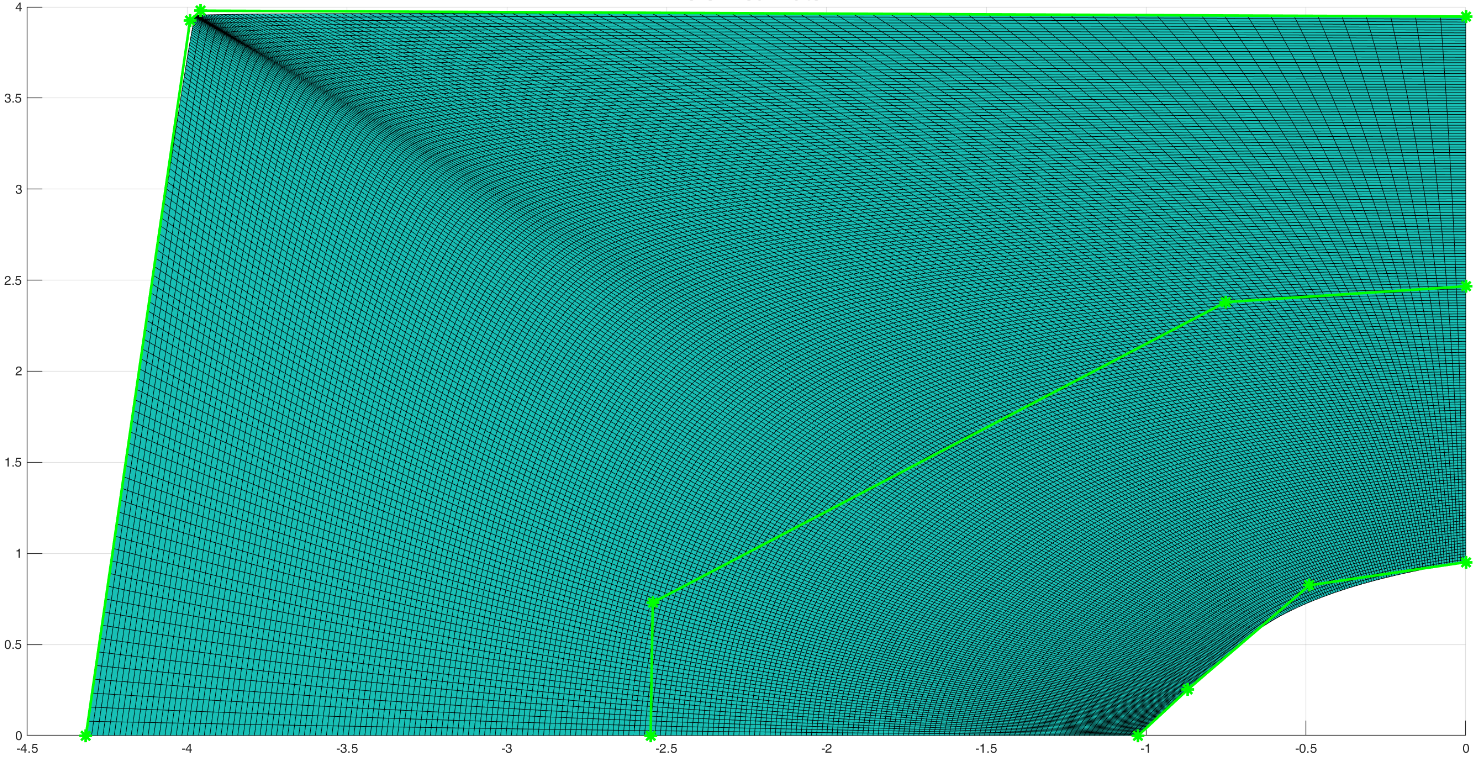
\includegraphics[width=1.0\textwidth,height=0.5\textheight]{figures/deformed_plate.png} \\
    \centering \label{Deformed Plate}
  \end{minipage}
      \item The nodal displacement vector is obtained using the following equation.
      \item $ [K^G] \{U\} = \{F^G\}$ 
      \item The displacements are then added to the control points and the new control points are then used to plot the deformed plate.
\end{itemize}

\end{frame}

%%%%%%%%%%%%%%%%%%%%%%%%%%%%%%%%%%%%%%%%%%%%%%%%%%%%%%%%%%%%%%%%%%%%%%
% Concluding remarks
%%%%%%%%%%%%%%%%%%%%%%%%%%%%%%%%%%%%%%%%%%%%%%%%%%%%%%%%%%%%%%%%%%%%%%

\section{Conclusions}
\begin{frame}[allowframebreaks] \frametitle{Conclusions}
  \begin{itemize}
      \item B-spline basis function has unique properties like local support, exact geometry representation and refinement techniques.
      \item IGA analysis framework makes use of these NURBS properties.
      \item Coupling of CAD and analysis solvers reduces the burden of mesh regeneration.
      \item This minimizes the computational cost
      \item Utilizing exact geometry in analysis provide accurate results than FEA. 
      \item Multi-patch B-spline modelling of intricate shapes ia very difficult task.
      \item Irrespective of the degree of basis function or no. of elements, FEA gives exact solution at node, but not IGA because of non-interpolation of B-spline control points      
  \end{itemize}
\end{frame}

%%%%%%%%%%%%%%%%%%%%%%%%%%%%%%%%%%%%%%%%%%%%%%%%%%%%%%%%%%%%%%%%%%%%%%
% References and question
%%%%%%%%%%%%%%%%%%%%%%%%%%%%%%%%%%%%%%%%%%%%%%%%%%%%%%%%%%%%%%%%%%%%%%

\begin{frame}
  
  % git repo link  
  \begin{columns}
    \column{6cm}
    \begin{block}{\centering{\huge  Any Questions?}}
      \centerline{ 
        
\includegraphics[width=0.5\textwidth]{figures/questions.png} 
      }
    \end{block}
  \end{columns}
  
\end{frame}

\end{document}
